% ---------------------------------------------------------------------
% -------------- PREAMBLE ---------------------------------------------
% ---------------------------------------------------------------------

%\documentclass[12pt,a4paper,finnish,oneside]{article}
\documentclass[lnbip]{svmultln}

\usepackage[utf8]{inputenc}
\usepackage[english]{babel}

\usepackage{calc}      % käytetään laskurien (counter) yhteydessä (tiedot.tex)
\usepackage{natbib}
\usepackage{url}
\usepackage{listings}
\usepackage{hyphenat}

\usepackage{supertabular,array}
\usepackage{lipsum}
\usepackage{booktabs}
\usepackage{graphicx}


% Strikethrough
\usepackage[normalem]{ulem}

% Punctuation for references
\bibpunct{[}{]}{;}{n}{,}{,}

% correct bad hyphenation here
\hyphenation{op-tical net-works semi-conduc-tor}


\usepackage{multibib}
\newcites{gen}{References}
\usepackage{bibentry}


% ---------------------------------------------------------------------
% -------------- DOCUMENT ---------------------------------------------
% ---------------------------------------------------------------------

\begin{document}

\selectlanguage{english}

\mainmatter


\title{Adopting agile in the large: motivations, success factors and challenges}

\titlerunning{Adopting agile in the large}

\author{Kim Dikert \and Maria Paasivaara \and Casper Lassenius}
\authorrunning{Kim Dikert et al.}   % abbreviated author list (for running head)

% list of authors for the TOC (use if author list has to be modified)
\tocauthor{Kim Dikert, Maria Paasivaara, Casper Lassenius}

\institute{Aalto University . . . Address . . .
\\ \email{kim.dikert@aalto.fi}, \email{maria.paasivaara@aalto.fi} }

\maketitle


% ---------------------------------------------------------------------
% -------------- ABSTRACT AND TEXT ------------------------------------
% ---------------------------------------------------------------------

\begin{abstract}        % give a summary of your paper
Abstract: miksi on tärkeätä tutkia tätä?
-- Mitkä on pääasialliset löydökset?
The abstract should summarize the contents of the paper
using at least 70 and at most 150 words. It will be set in 9-point
font size and be inset 1.0 cm from the right and left margins.
There will be two blank lines before and after the Abstract.
%                         please supply keywords within your abstract
\keywords {agile, transformation, large scale, adopting agile}
\end{abstract}


% ---------------------------------------------------------------------
\section{Introduction}

As the competition in software industry is growing companies are constantly
looking to improve their effectiveness. Agile methods are claimed to increase
productivity and quality \citegen{Livermore2008}, which makes them attractive for
companies pursuing better performance. However, large organizations may have
problems introducing agile methods \citegen{Dyba2009}. As agile methods are
initially designed for small teams their application has proven to be
problematic in a larger scale \citegen{Boehm2005}.

It is typical for large companies to function according to plan-driven software
engineering models. These models strive for consistent quality and performance
by rigorous planning and definition of process. This kind of approach is however
badly suited for software development, as projects typically encounter
situations that are too hard or impossible to foretell \citegen{Schwaber2002}.
The main problems in plan-driven development are the high cost of changes and
late feedback on quality \citegen{Petersen2010}. Long release cycles, cost of
responding to change and distance from customers undermine the  competitiveness
of companies. Agile methods are believed to bring remedy to these problems.

The goal of this research is to explore how and why large organizations adopt
agile methods. Studies on large scale agile transformations have been published,
but no extensive or summarizing research is available on the subject. In this
research we will give an overview of reported case studies on adopting agile
methods in large organizations. We will further discuss the motivations for
adopting agile methods, the characteristics of agile transformations, and
factors relating to success or challenge in the transformation process. Our
research is focused on the process of organizational change. We leave out topics
related to comparing the initial and transformed states of organizations, such
as measuring the performance of organizations before and after the
transformation.

This paper is organized as follows. The next section gives an overview of large
scale agile development. Section \ref{sec:method} presents the literature review
method used for conducting this research. The findings of the review are
discussed in section \ref{sec:results}, and section \ref{sec:conclusion}
presents limitations and proposals for future research.


% ---------------------------------------------------------------------
\section{Background}
\label{sec:background}

Introducing agile methods in large organizations is more difficult than it is in
small organizations \citegen{Dyba2008}. The difficulty is partly related to size
bringing higher organizational inertia which slows down organizational change
\citegen{Livermore2008}. Agile methods are not founded on the use of individual
tools or practices, but rather on a holistic way of thinking.
Adopting agile requires often change of the entire organizational culture
\citegen{Misra2010}.

One significant difference between small and large adoptions is that large
organizations have more dependencies between projects and teams. This increases
the need for formal documentation and thus reduces agility \citegen{Lindvall2004}.
In addition to inter-team coordination development teams are required to
interact with other organizational units, which are often non-agile of their
nature. For instance, HR may demand individuals to have strictly specified roles
in projects \citegen{Boehm2005}, or a change control board may inhibit use of
continuous integration or refactoring \citegen{Lindvall2004}. All units affected
by the agile transformation need to be informed and heard, and the agile process
must be adjusted according to their needs \citegen{Lindvall2004, Cohn2003,
Boehm2005}.

Agile methods will also affect management and business related functions. A key
challenge is that management must move away from life cycle models and towards
iterative and feature centric models \citegen{Nerur2005}. The focus must be
shifted from a large scale scope to shorter term project planning
\citegen{Misra2010}, as agile methods emphasize that planning is only meaningful
for the near future \citegen{Cohn2003}. However, the lack of planning can be a
concern as business and customer relationships often build on long term
roadmapping. Enabling operation with shorter term planning requires educating
stakeholders and reviewing contracting practices \citegen{Boehm2005}.


% ---------------------------------------------------------------------
\section{Research method}
\label{sec:method}

% Research questions:
%
% What are the motivations for starting an organizational transformation?
%
% What kind of agile transformations have been reported?
%
% What were challenges and success factors in the transformation process?


The literature review was conducted as an application of Kitchenham's
method for systematic literature review (SLR) \citegen{Kitchenham2007}. The method
was applied to be performed by only one researcher, and to serve as a
preliminary work evaluating the feasibility of a more in-depth review.
Effort was limited by selecting only the following subset of SLR steps:
identification of primary sources, data extraction and synthesis. Steps left out
were the development of a systematic review protocol, strict study quality
assessment, and reviews in the study selection process.

The searches for primary sources was conducted in two steps. First a preliminary
search was made to sample the existing literature. Then a systematic search was
done based on the preliminary search. The following databases were included in
the searches: IEEExplore (http://ieeexplore.ieee.org/),
ACM (http://dl.acm.org/), Scopus (http://www.scopus.com/),
ProQuest \linebreak (http://search.proquest.com/).
Additionally the archive of International XP
Conference (http://link.springer.com/) was searched.

The search phrases used in the preliminary search were \textit{agile
transformation} and \textit{large scale agile}. For the systematic search three
facets and appropriate keywords were chosen, as presented in Table
\ref{table:searchterms}. To search the databases a query phrase was constructed
by joining the keywords of each facet by \texttt{OR} operators and the facets by
\texttt{AND} operators.

As the preliminary search omitted some of the keywords in Table
\ref{table:searchterms} it yielded a small number of additional matches. The
reason for variance in matches was that many articles had creative titles or the
abstracts and keywords were not informative enough. Because of this, the search
with more restrictive keywords was unable to capture all possible matches.
We are however confident that the search covered the majority of material
relating to agile transformations in large organizations. If a wider search
should be performed, our recommendation is to only regard the facets
\textit{agile methods} and \textit{organizational change}. This would lead to
significantly more matches in the first stage of selecting studies, but the
additional effort is necessary due to the limitations of a keyword search.

\begin{table}[t]
    \begin{tabular}{ l@{ \hskip 0.4cm } l }
        \toprule
        Facet                  & Keywords   \\ \midrule
        Agile methods          & agile, scrum, lean, xp \\ 
        Organizational change  & transformation, transition, change, migration \\
        Large organization     & enterprise, organization, (large \texttt{AND} scale) \\
        \bottomrule
    \end{tabular}
    \caption{Facets and related search terms used}
    \label{table:searchterms}
\end{table}

\begin{figure}[b]
  \begin{center}
    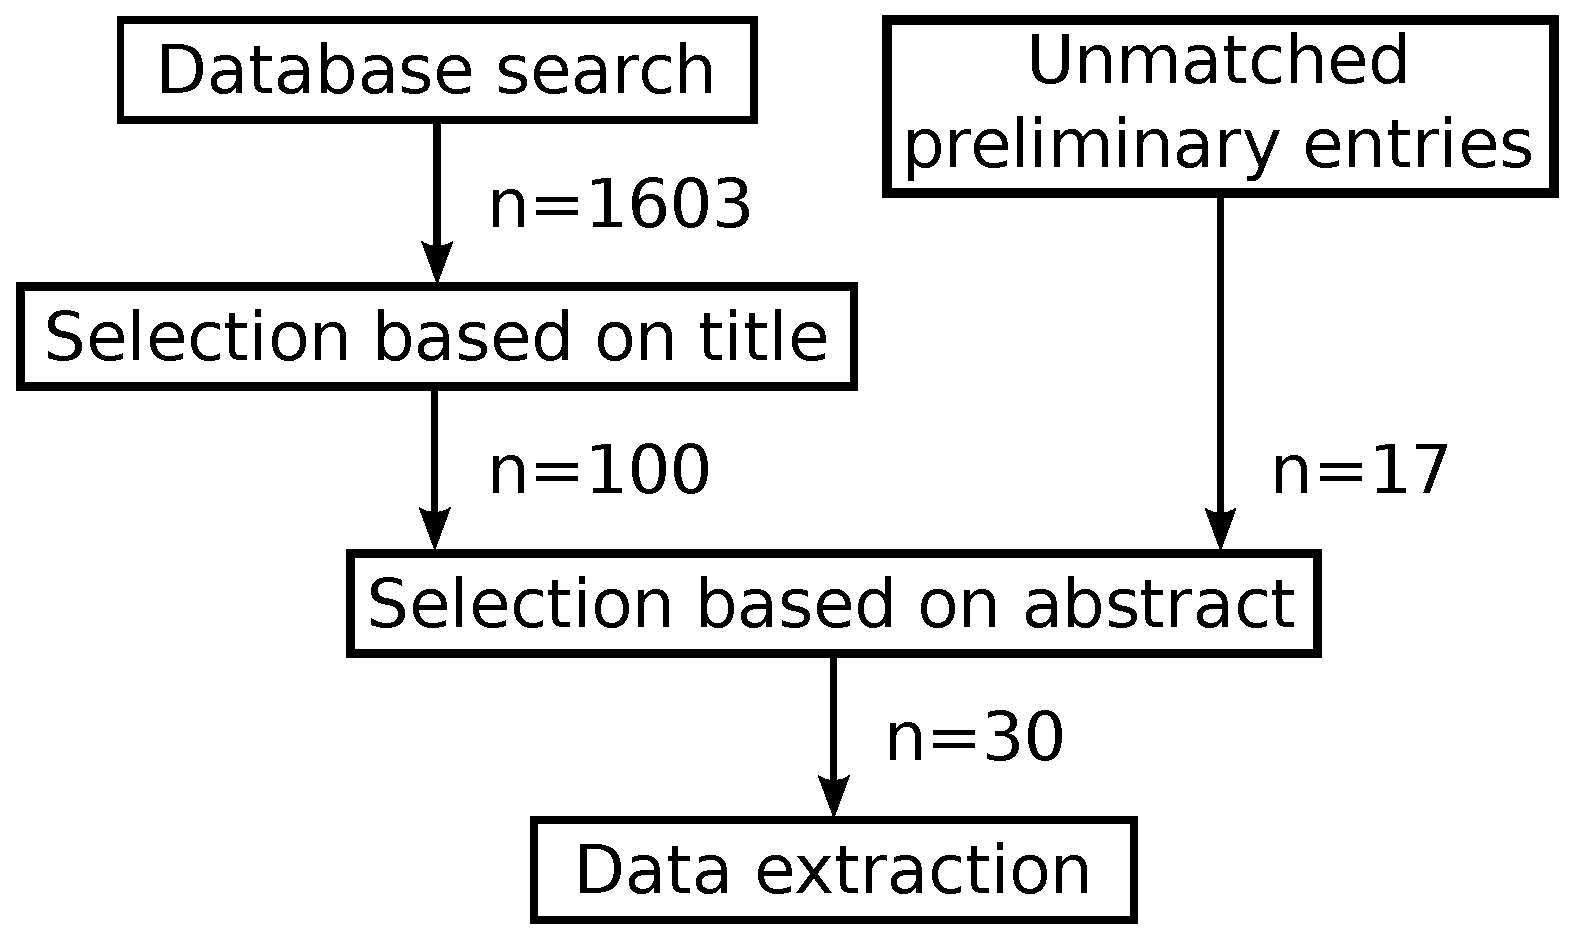
\includegraphics[width=0.45\textwidth]{researchprocess}
    \caption{Process of selecting primary studies}
    \label{fig:selection_process}
  \end{center}
\end{figure}

The selection process of the primary studies is summarized in Figure
\ref{fig:selection_process}. The database search yielded 1603 matches which were
filtered down to 31 selected primary studies. One study was not available, which
reduced the final number of primary studies to 30.
The 30 primary sources were selected by four criteria: study type, size of
organization, use of agile methods in software development, and a transformation
viewpoint. Firstly, only case studies and experience reports on agile software
development were included in this study. Papers discussing agile methods or
organizational transformation on as a general topic were left out. Secondly, the
size of the organization described in the included primary studies was to be
large enough to show the challenges of large scale agile development
\citegen{Lindvall2004}. Further, only studies discussing agile software
development were included, leaving out for instance studies on agile management.
Finally, the included studies had to provide a viewpoint on the adoption of
agile methods.

%\subsection{Data extraction}

Analysis of the primary studies was guided by using a data extraction form with
open ended fields. The reason for starting a transformation was captured in
fields \textit{initial state of organization} and \textit{reasons for change}.
The description of the transformation process was captured in one field.
Recommendations for transformation processes were captured in fields
\textit{reported good practices}, \textit{reported challenges}, and
\textit{lessons learned}.
Additional fields that were used but not sufficiently answered by the primary
studies were \textit{satisfaction after transformation} and \textit{reported
measurements before/after transformation}.


% ---------------------------------------------------------------------
\section{Results}
\label{sec:results}

Of the 30 included primary studies 23 were experience reports and 7 were case
studies. From a validity viewpoint it is important to acknowledge that most of
the studies were written by employees in the studied organizations.

\begin{figure}[b]
  \begin{center}
    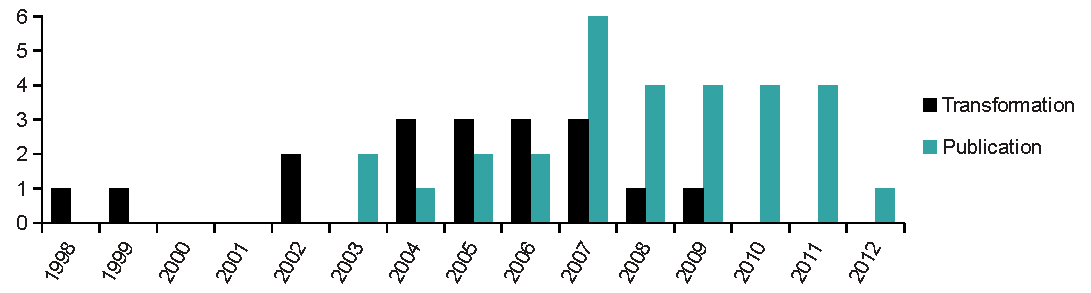
\includegraphics[width=1\textwidth]{publicationschart.pdf}
    \caption{Time of publications and transformations}
    \label{fig:publications}
  \end{center}
\end{figure}

All of the included studies had been published within a decade. On average the
studies were published three years after the transformation was reported to
have begun. Figure \ref{fig:publications} gives a timeline view of the
publications.

The most commonly reported methods are listed in Table \ref{table:methods}, of
which Scrum was the most popular single method. An important observation is that
tailoring of methods was very common. The use of tailoring can be considered
relating particularly to large scale, as the core of agile methods give very
little advice on interfacing with other units present in a large organization.
The agile team must interface with units such as other development teams,
management, and marketing.

\begin{table}[t]
    \begin{tabular}{ l@{ \hskip 0.4cm } l }
        \toprule
        Agile method    & Reported in number of studies   \\ \midrule
        Scrum           & 18 \\ 
        XP              & 7 \\
        Lean            & 5 \\
        Tailoring and combining methods & 9  (indirect mentioning not counted) \\
        \bottomrule
    \end{tabular}
    \caption{Reported use of agile methods}
    \label{table:methods}
\end{table}


The reasons to initiate a change fell into three categories, as summarized in
Table \ref{table:motivations}. The primary reasons for change was a strategical
need to improve the performance of the organization. Especially shortening the
time to market was desired. In many cases the change was started when management
acknowledged problems in the current way of working.

\begin{table}[t]
    \begin{tabular}{ l@{ \hskip 0.4cm } l }
        \toprule
        Reason                                    & In studies   \\ \midrule
        Need to improve performance               & S8, S11, S15, S16, S17, S24, S27 \\ 
        Need to improve time to market            & S6, S9, S13, S19, S24 \\
        Need to eliminate known process problems  & S5, S6, S10, S13, S19, S21 \\
        \bottomrule
    \end{tabular}
    \caption{Reported reasons for initiating a transformation}
    \label{table:motivations}
\end{table}


The most usual way of implementing the change was a stepwise adoption of agile,
which usually included a pilot project. A typical stepwise adoption was to first
create agile teams and introduce basic practices. Having intra-team agile
practices in place made it possible to see how the entire organization would be
affected by the agile way of working.

The central role of management in the change was evident in many studies. This
was typically shown in that the change was initiated by the management and
management took responsibility of the change process. Several studies identified
a champion who was the driver of the change. Some studies reported the change to
be driven by external consultants or a cross organizational work group.

Typical challenges and and success factors reported in the studies are listed in
Table \ref{table:success}. In both cases the ability to align the organization
was a central factor in both cases. Challenges surface if not everyone is on
board with the change. Good ground for the change is created by strongly
communicating a clear vision and enabling everyone to participate. Resourcing
for the change was also seen both as a challenge and a success factor.
The studies show that allocating extra training and hiring of external consultants
facilitate the change.

A particular challenge for adopting agile was misunderstanding how agile should
be applied. Some symptoms of this were talking agile but still working the old
way, and managers making commitments without hearing development teams.
As expected, many studies reported that teams had problems interfacing with
other organizational units, such as management and marketing.

It is difficult to make a new way of working stick in a large organization.
Use of agile can be rooted into the organization by creating an agile community.
Founding of interest groups and arranging regular seminars are good ways for
building community. As agility emphasizes people centricity and flexibility the
new ways of working can not be mandated. Instead, coaching should be applied for
leading the change. Several studies suggest conformity in the application of
agile models. Conformity avoids disorder when several teams are simultaneously
finding their agile ways.

\begin{table}[t]
    \begin{tabular}{ p{0.31\textwidth} p{0.67\textwidth} }
        \toprule
        Class of challenge  & Examples   \\ \midrule
        
        \raggedright Aligning organization for change  &
             Lack of management support [S1, S5, S13]\newline
             Change resistance [S14, S22, S26] \newline
             Reverting to old model [S4, S11, S23] \\ 
        
        \raggedright\rule{0pt}{0.4cm}Misunderstanding the agile model  &
             Wrong application of roles and responsibilities \newline
             [S11, S13, S16, S17, S23, S24] \newline
             Agile terms merely mask the old model [S10, S22] \\
        
        \raggedright\rule{0pt}{0.4cm}Effect of agile outside of development  &
            Conflicts with business (e.g. planning) [S6, S11, S21] \newline
            Making non-development functions agile (testing, maintenance, etc.) [S2, S4, S13]\newline
            Conflicts with other units (marketing, HR, etc.) \newline[S6, S10, S11, S13] \\
        
        \raggedright\rule{0pt}{0.4cm}Lack of resources  &
            Lack of training, insufficient resources for coaching \newline
            [S5, S13, S22, S28]\\
        
        \midrule
        Class of success factors  & Examples   \\ \midrule
        
        \raggedright Organization alignment and leadership  &
             Management support [S8, S9, S10, S13, S16, S19] \newline
             Communicate vision for new process [S7, S19] \newline
             Demand all organizational units to participate [S13, S15, S17, S18, S19, S21] \\ 
        
        \raggedright\rule{0pt}{0.4cm}Coaching and community  &
             Create community to make change stick [S6, S7, S19, S28] \newline
             Lead change by a coaching approach [S1, S4, S22, S28] \\
        
        \raggedright\rule{0pt}{0.4cm}Tailoring and conformity  &
            Tailor the most suitable model [S8, S11, S20] \newline
            Conformity clarifies use of new model [S19, S24, S29, S30]\\
        
        \raggedright\rule{0pt}{0.4cm}Investing in change  &
            Training, consulting, physical spaces, tools [S6, S14, S19]\\
        \bottomrule
    \end{tabular}
    \caption{Challenges and success factors reported in studies}
    \label{table:success}
\end{table}


% ---------------------------------------------------------------------
\section{Limitations and future research}
\label{sec:conclusion}

The papers included in this study were mostly experience reports with no
research method. Some papers were of low quality, but they were included as our
aim was to give a view of the topic that is broader and inclined towards practice.

Differing from our initial beliefs, this research shows that a body of studies
on large scale agile transformations has emerged. We aim to continue our
research on this topic by conducting a systematic literature review. Beyond
descriptive reports on agile transformations we found very little studies with
quantitative comparison of organizations' performance before and after the
transformations.


% \subsection{TODO}


% Vielä:
% Missä sanotaan mikä on "large"
% Success factor: Stepwise adoption (piloting)


% Pitäs olla done:
% Search kuva on selitetty myös tekstissä.
% Inclusion: viewpoint on the organizational transformation [from plan-driven, tms.]
% Used methods: interfacing with various units present in a large organization
%    --> Developmentin koordinointi
% "Coaching and community" --> selitä myös coaching


% ---------------------------------------------------------------------
% -------------- BIBLIOGRAPHY -----------------------------------------
% ---------------------------------------------------------------------

%\small
\fontsize{9pt}{10pt}\selectfont

\bibliographystyle{plain}
\bibliographystylegen{plain}

\bibliographygen{sources}

\nobibliography{sources_s}

\subsection*{Primary studies}


\begin{supertabular}{ l p{11.4cm} }
    {[}S1{]} & \bibentry{S1} \\  \shrinkheight{-1cm}
    {[}S2{]} & \bibentry{S2} \\ 
    {[}S3{]} & \bibentry{S3} \\ 
    {[}S4{]} & \bibentry{S4} \\ 
    {[}S5{]} & \bibentry{S5} \\ 
    {[}S6{]} & \bibentry{S6} \\ 
    {[}S7{]} & \bibentry{S7} \\ 
    {[}S8{]} & \bibentry{S8} \\ 
    {[}S9{]} & \bibentry{S9} \\
    {[}S10{]} & \bibentry{S10} \\ 
    {[}S11{]} & \bibentry{S11} \\ 
    {[}S12{]} & \bibentry{S12} \\  \shrinkheight{-1.4cm}
    {[}S13{]} & \bibentry{S13} \\ 
    {[}S14{]} & \bibentry{S14} \\ 
    {[}S15{]} & \bibentry{S15} \\ 
    {[}S16{]} & \bibentry{S16} \\ 
    {[}S17{]} & \bibentry{S17} \\ 
    {[}S18{]} & \bibentry{S18} \\ 
    {[}S19{]} & \bibentry{S19} \\ 
    {[}S20{]} & \bibentry{S20} \\ 
    {[}S21{]} & \bibentry{S21} \\ 
    {[}S22{]} & \bibentry{S22} \\ 
    {[}S23{]} & \bibentry{S23} \\ 
    {[}S24{]} & \bibentry{S24} \\ 
    {[}S25{]} & \bibentry{S25} \\ 
    {[}S26{]} & \bibentry{S26} \\ 
    {[}S27{]} & \bibentry{S27} \\ 
    {[}S28{]} & \bibentry{S28} \\ 
    {[}S29{]} & \bibentry{S29} \\ 
    {[}S30{]} & \bibentry{S30} \\ 
\end{supertabular}\end{document}
